%% sections/06-spectral-clustering.tex
%% Section 4: Spectral Clustering. Split out of the spiked-covariance section
%% so the application stands on its own. 4.1 derives the Gram matrix as a
%% spiked model (two theorems + synthetic studies); 4.2 tests it on MNIST.

\section{Spectral Clustering}\label{sec:clustering}

Everything so far has concerned one kind of hidden structure: a few directions along which the data vary more than the noise. Clustering asks about another.

\subsection{From Spiked Covariance to Spectral Clustering}\label{subsec:clustering}

We observe \(n\) independent \(p\)-vectors drawn from \(K\) classes,\gdmark{r4-clustering-intro}
\begin{equation}
  \vect{x}_i \;=\; \vect{\mu}_{k(i)} \;+\; \vect{w}_i, \qquad \{\vect{w}_i\}_{i=1,\dots,n} \stackrel{\textnormal{i.i.d.}}{\sim} \Normal{\vect{0}, I_p},
  \label{eq:clustering-model}
\end{equation}
where \(\vect{\mu}_k\) is the unknown mean of class \(k\) and \(k(i) \in \{1, \dots, K\}\) is the class of observation \(i\). The goal of \vocab{clustering} is to estimate the labels \(k(i)\) with no parameter of the model known in advance, \(K\) included (some methods do assume \(K\); ours does not).\gdmark{r4-clustering-goal} Following \citet{LebeauChatelainCouillet2024}, we show that the spiked-model machinery of the previous section solves it.

\paragraph{The model in matrix form.}
Stack the observations as columns of \(\mat{X} \in \R^{p \times n}\), the group means as columns of \(\mat{M} = (\vect{\mu}_1 \mid \cdots \mid \vect{\mu}_K) \in \R^{p \times K}\), and record the assignments in the \vocab{assignment matrix} \(\mat{J} \in \{0, 1\}^{n \times K}\), with \(J_{i k} = 1\) if observation \(i\) belongs to group \(k\) and \(0\) otherwise. Each row of \(\mat{J}\) has exactly one \(1\), and recovering \(\mat{J}\) is the goal of clustering.\gdmark{r4-bookkeeping} In matrix form, the model becomes
%then reads
\begin{equation}
  \mat{X} \;=\; \underbrace{\mat{M} \mat{J}\transpose}_{\text{signal } \mat{P}} \;+\; \underbrace{\mat{W}}_{\text{noise}},
  \label{eq:clustering-matrix}
\end{equation}
where \(\mat{W}\) is a \(p \times n\) matrix of i.i.d.\ \(\Normal{0, 1}\) entries. The signal \(\mat{P} = \mat{M}\mat{J}\transpose\) has rank at most \(K\): a low-rank term added to full-rank noise. This is the same mathematical shape as the spiked model, a low-rank perturbation of a noise matrix, though here the structure lives in the column means rather than in a covariance.\gdmark{r4-lowrank}

It is convenient to normalize the factorization. Let \(n_k\) be the size of group \(k\) and \(\mat{D} = \diag(n_1, \dots, n_K)\). Writing
\begin{equation}
  \mat{P} \;=\; \mat{L} \mat{V}\transpose, \qquad \mat{L} = \mat{M} \mat{D}^{1/2}, \qquad \mat{V} = \mat{J} \mat{D}^{-1/2},
  \label{eq:LV-factorisation}
\end{equation}
the columns \(\vect{v}_1, \dots, \vect{v}_K\) of \(\mat{V}\) are orthonormal: \(\vect{v}_k\) has entries \(1/\sqrt{n_k}\) on the members of group \(k\) and \(0\) elsewhere. We call them the \vocab{normalized indicator vectors}. They are the cleanest possible encoding of the answer: knowing the \(\vect{v}_k\) (even approximately, even in scrambled order) is knowing the clusters.

\paragraph{The similarity matrix.}
Spectral clustering works not with \(\mat{X}\) itself but with an \(n \times n\) \vocab{similarity matrix} whose \((i, j)\) entry measures how alike observations \(i\) and \(j\) are.\gdmark{r4-similarity} The simplest choice is the \vocab{Gram matrix}
\[
  \mat{G} \;=\; \frac{1}{p}\, \mat{X}\transpose \mat{X}, \qquad G_{i j} \;=\; \frac{1}{p} \inner{\vect{x}_i}{\vect{x}_j}.
\]
Note the reversal: \(\Sigmahat_n = (1/n)\mat{X}\mat{X}\transpose\) is \(p \times p\) and built from pairs of features, while \(\mat{G}\) is \(n \times n\) and \(G_{ij}\) is the similarity between data points \(i\) and \(j\).\gdmark{r4-reversal} An eigenvector of \(\mat{G}\) therefore has one entry per data point, the right shape for an object meant to label them.\gdmark{r4-kernels-cut}

Two facts connect \(\mat{G}\) to what we have done. First, with no signal (\(\mat{P} = \vect{0}\)) the Gram matrix is \(\mat{G} = (1/p)\mat{W}\transpose\mat{W}\). For any matrix, \(\mat{W}\transpose\mat{W}\) and \(\mat{W}\mat{W}\transpose\) share their nonzero eigenvalues (multiply \(\mat{W}\mat{W}\transpose\vect{u} = \lambda\vect{u}\) by \(\mat{W}\transpose\)), so \((1/p)\mat{W}\transpose\mat{W}\) and \((1/n)\mat{W}\mat{W}\transpose\) share theirs up to the factor \(n/p = 1/y\). These two are \emph{companion matrices}: the empirical spectral distribution of \((1/n)\mat{W}\mat{W}\transpose\) converges to the Marchenko-Pastur law of Section~\ref{subsec:scm-highdim}, so the spectrum of \(\mat{G}\) converges to that law rescaled by \(1/y\),\gdmark{r4-noise-part} with edges
\[
  \frac{\lambda_\pm}{y} \;=\; \frac{(1 \pm \sqrt{y})^2}{y} \;=\; \Bigl(\frac{1}{\sqrt{y}} \pm 1\Bigr)^{2},
\]
together with \(n - p\) zero eigenvalues when \(p < n\), since \(\mat{G}\) has rank at most \(p\). Second, adding the signal \(\mat{P}\) is a low-rank perturbation whose eigenvectors carry the clusters: the noiseless similarity matrix \((1/p)\mat{P}\transpose\mat{P} = \mat{V}\bigl[(1/p)\mat{L}\transpose\mat{L}\bigr]\mat{V}\transpose\) has eigenvectors that combine the normalized indicators \(\vect{v}_k\), and when the means are orthogonal they \emph{are} the indicators. Whether the top eigenvectors of \(\mat{G}\) stay close to this structure once noise is added is precisely a spiked-model question, which the next two theorems answer.\gdmark{r4-signal-streamline}

\paragraph{The two theorems.}
The strength of group \(k\)'s signal is measured by the eigenvalues \(\ell_1 \ge \cdots \ge \ell_K \ge 0\) of the \(K \times K\) matrix \((1/n)\mat{L}\transpose\mat{L}\); for orthogonal means, \(\ell_k = \norm{\vect{\mu}_k}^2 \cdot n_k / n\), so \(\ell_k\) is simply a signal-to-noise ratio. (When the means are linearly dependent, as in the \(\pm\vect{\mu}\) design of study~(a) below, some \(\ell_k\) vanish and the signal carries correspondingly fewer spikes.) The first theorem is the clustering analogue of the spike phase transition of Theorem~\ref{thm:bbp}, with the threshold now at \(\sqrt{y}\).

\begin{theorem}[Spikes of the Gram matrix, {\citealp[Thm.~1]{LebeauChatelainCouillet2024}}]\label{thm:gram-spikes}
In model~\eqref{eq:clustering-matrix}, assume the group sizes stay comparable, the positive \(\ell_k\) are distinct, and \(p, n \to \infty\) with \(p/n \to y \in (0, \infty)\). Let \((\lambda_k, \widehat{\vect{v}}_k)\) be the \(k\)-th largest eigenvalue-eigenvector pair of \(\mat{G}\), and let \(\vect{v}_k\) now denote the eigenvector of the noiseless similarity matrix \((1/p)\mat{P}\transpose\mat{P}\) attached to its \(k\)-th largest eigenvalue (for orthogonal means this is exactly the \(k\)-th normalized indicator). Then, for each \(k\) with \(\ell_k > 0\),
\[
  \lambda_k \;\convas\;
  \begin{cases}
    \xi_k \;=\; \dfrac{(\ell_k + y)(\ell_k + 1)}{y\, \ell_k} & \text{if } \ell_k > \sqrt{y}, \\[1.2em]
    \Bigl(1 + \dfrac{1}{\sqrt{y}}\Bigr)^{2} & \text{otherwise},
  \end{cases}
  \]
  \[
  \abs{\inner{\vect{v}_k}{\widehat{\vect{v}}_k}}^2 \;\convas\;
  \begin{cases}
    \zeta_k \;=\; 1 - \dfrac{\ell_k + y}{\ell_k (\ell_k + 1)} & \text{if } \ell_k > \sqrt{y}, \\[1.2em]
    0 & \text{otherwise}.
  \end{cases}
\]
\end{theorem}

The statement is proved in \citet[][Thm.~2]{CouilletChatelainLeBihan2021}, and every feature is familiar. A signal direction whose signal-to-noise ratio clears \(\sqrt{y}\) produces an isolated eigenvalue at \(\xi_k\) outside the bulk and an eigenvector that aligns with its population counterpart to the definite degree \(\zeta_k < 1\); one below the threshold is absorbed into the bulk and its eigenvector carries no information, exactly the fundamental versus non-fundamental dichotomy of Sections~\ref{subsec:bbp} and~\ref{subsec:eigenvector}. Even the fine structure repeats: the map \(\ell \mapsto \xi\) has derivative \(1/y - 1/\ell^2\), which vanishes exactly at \(\ell = \sqrt{y}\), so the outlier leaves the bulk edge flatly, the same tangency that made the critical window of Section~\ref{subsec:fluctuations} delicate.

The second theorem is the one our Section~\ref{subsec:eigenvector} could not offer for the covariance model. There we measured eigenvectors only through limiting \emph{constants}; the raw alignment converges to a number, so its limiting distribution is degenerate, and to see an honest limit law one must first center and then rescale. The following result does exactly that, one entry at a time.

\begin{theorem}[Entrywise fluctuations, {\citealp[Thm.~2]{LebeauChatelainCouillet2024}}]\label{thm:eigvec-clt}
In the setting of Theorem~\ref{thm:gram-spikes}, fix \(k\) with \(\ell_k > \sqrt{y}\), fix the sign of \(\widehat{\vect{v}}_k\) by \(\inner{\vect{v}_k}{\widehat{\vect{v}}_k} \ge 0\), and let \(\mathcal{I} \subseteq \{1, \dots, n\}\) be any finite set of entries. Then
\[
  \frac{\sqrt{n}\, \bigl[\widehat{\vect{v}}_k - \sqrt{\zeta_k}\, \vect{v}_k\bigr]_{\mathcal{I}}}{\sqrt{1 - \zeta_k}}
  \;\convd\; \Normal{\vect{0},\, I_{\abs{\mathcal{I}}}}.
\]
\end{theorem}

Read entry by entry, Theorem~\ref{thm:eigvec-clt} says
\begin{equation}
  [\widehat{\vect{v}}_k]_i \;\approx\; \Normal{\sqrt{\zeta_k}\, [\vect{v}_k]_i,\; \tfrac{1 - \zeta_k}{n}},
  \label{eq:entrywise}
\end{equation}
with distinct entries asymptotically independent: each entry of the sample eigenvector is the corresponding entry of the true indicator, shrunk by the factor \(\sqrt{\zeta_k}\) and blurred by Gaussian noise whose variance \((1 - \zeta_k)/n\) is exactly the alignment that is missing. The signal-plus-noise structure of the data matrix~\eqref{eq:clustering-matrix} is transferred intact to the eigenvector. The proof is short and elegant, and we sketch its two steps. First, the eigenvector decomposes as \(\widehat{\vect{v}}_k = \sqrt{\zeta_k}\, \vect{v}_k + \sqrt{1 - \zeta_k}\, \widehat{\vect{v}}_k^{\perp}\) up to a vanishing error, where \(\widehat{\vect{v}}_k^{\perp}\) is a unit vector orthogonal to all the population eigenvectors \(\vect{v}_1, \dots, \vect{v}_K\). Second, because the noise \(\mat{W}\) looks the same in every orthonormal basis (the rotational invariance of Corollary~\ref{cor:gaussian-rotation}, met again with the GOE in Section~\ref{sec:scm}), \(\widehat{\vect{v}}_k^{\perp}\) is uniformly distributed on the unit sphere of that orthogonal complement. And any fixed handful of coordinates of a uniform high-dimensional sphere vector is asymptotically Gaussian: a uniform sphere vector is a Gaussian vector divided by its length, and in high dimension the length concentrates \citep{Vershynin2018}. Nothing about the argument needs the noise to be Gaussian, only rotationally invariant, which is why the prediction survives contact with real data below.

\paragraph{From fluctuations to accuracy.}
Equation~\eqref{eq:entrywise} turns clustering performance into a Gaussian tail computation. Take the balanced two-group case with means \(\pm\vect{\mu}\), where the single informative direction is \(\vect{v}\) with entries \(\pm 1/\sqrt{n}\) and the natural rule assigns observation \(i\) to a group according to the sign of \([\widehat{\vect{v}}]_i\). By~\eqref{eq:entrywise}, an entry has mean \(\pm\sqrt{\zeta/n}\) and standard deviation \(\sqrt{(1-\zeta)/n}\), so it lands on the wrong side of zero with probability \(\Phi\bigl(-\sqrt{\zeta/(1-\zeta)}\bigr)\), where \(\Phi\) is the standard normal CDF. The expected fraction of correctly clustered points is therefore
\begin{equation}
  \text{accuracy} \;\approx\; \Phi\Bigl(\sqrt{\tfrac{\zeta}{1 - \zeta}}\Bigr),
  \label{eq:sign-accuracy}
\end{equation}
ranging from \(1/2\) (a coin flip) at \(\zeta = 0\) to perfect as \(\zeta \to 1\); a version for any number of groups is given in \citet{LebeauChatelainCouillet2024}. This was the missing piece: Theorem~\ref{thm:gram-spikes} alone says the eigenvector points partway at the truth, but only the fluctuation law says how many individual points end up on the wrong side.

\paragraph{Computational study (a): one fundamental spike.}
We test the chain end to end in the smallest instance: two balanced groups with means \(\pm \vect{\mu}\), which gives a rank-one signal with the single ratio \(\ell = \norm{\vect{\mu}}^2\), at \(y = 1/2\), \(n = 800\), \(p = 400\), \(\ell = 4\). Theorem~\ref{thm:gram-spikes} predicts an outlier at \(\xi = 11.25\) against a bulk ending at \((1 + \sqrt{2})^2 \approx 5.83\), and an alignment \(\zeta = 0.775\). Figure~\ref{fig:clustering-one-spike} confirms all three panels of the story: the spectrum is a rescaled MP bulk plus one spike at the predicted spot; the eigenvector entries form two bands at \(\pm\sqrt{\zeta/n}\), tracking the shrunken indicator with the predicted one-standard-deviation envelope; and the residuals match the predicted Gaussian \(\Normal{0, (1-\zeta)/n}\). The predicted accuracy~\eqref{eq:sign-accuracy} is \(\Phi(1.86) \approx 0.97\), visible in the middle panel as the small overlap of the two bands across zero.

\begin{figure}[H]
  \centering
  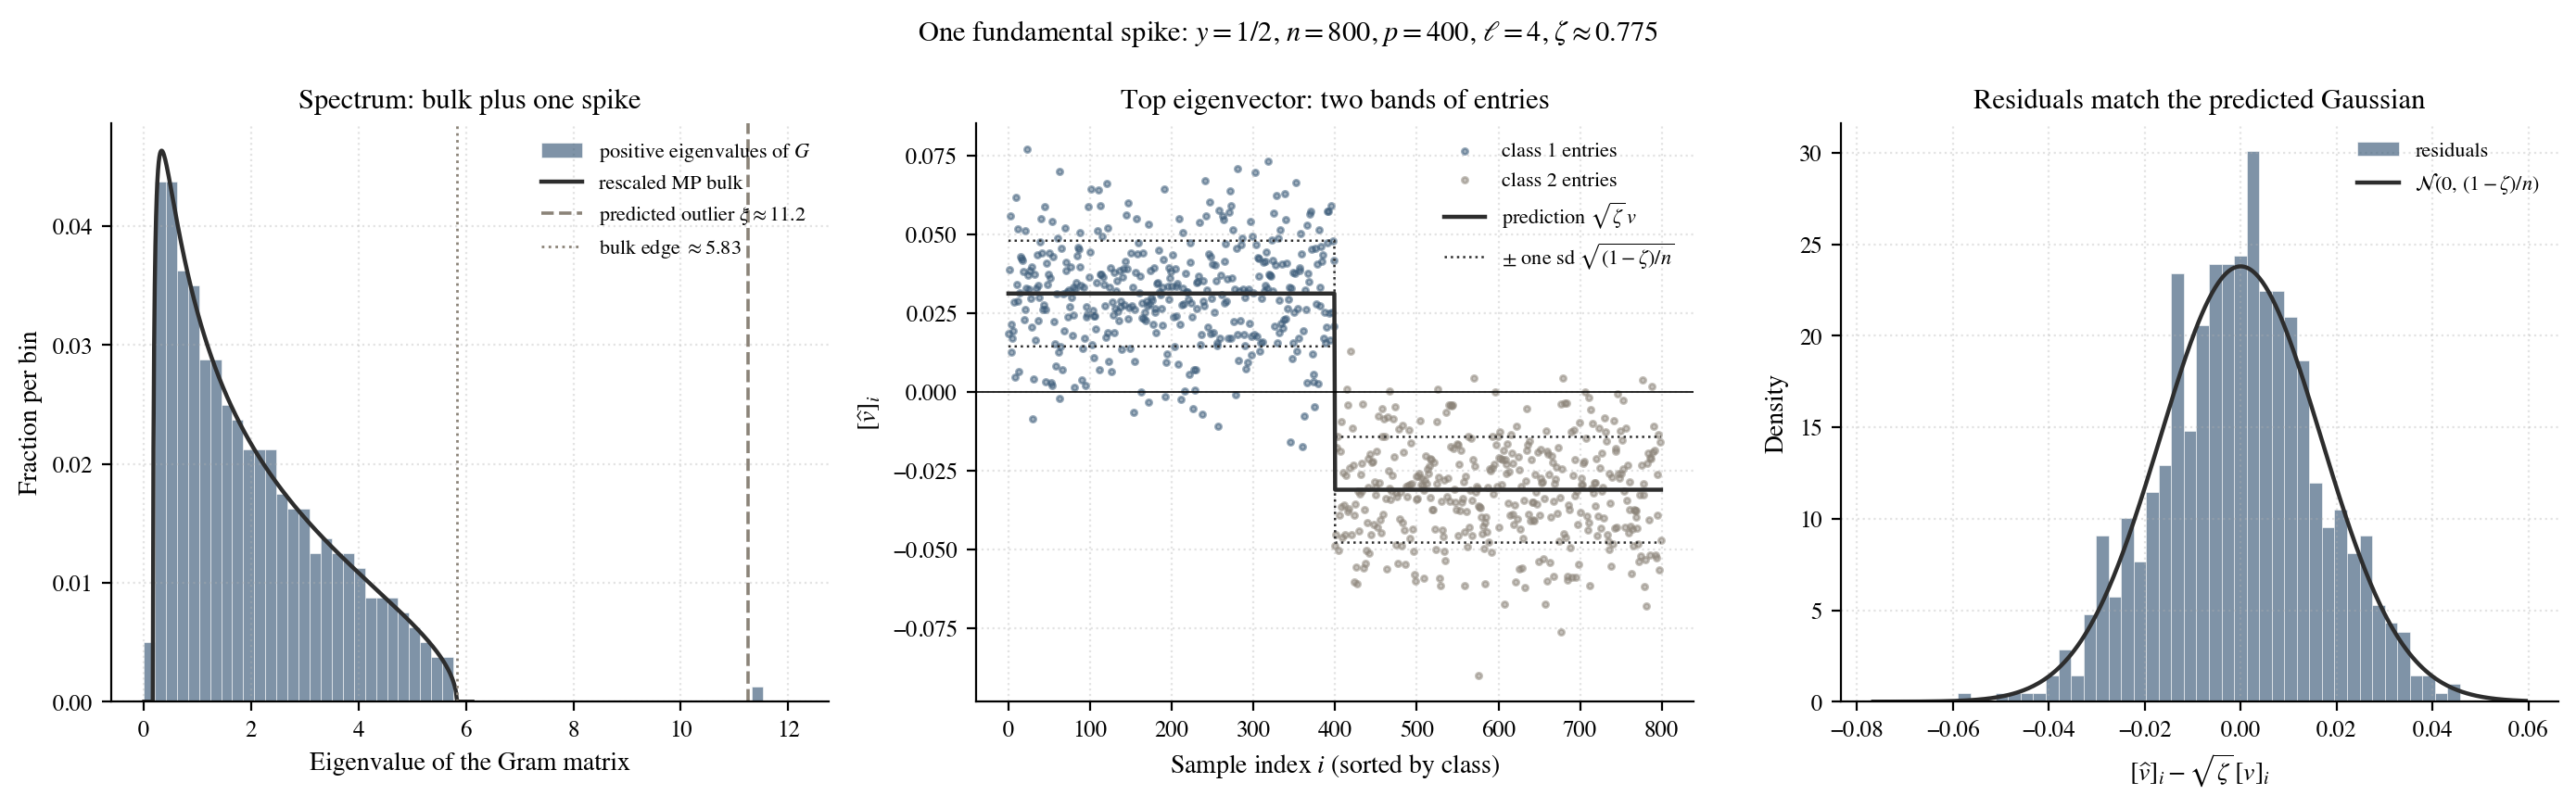
\includegraphics[width=\textwidth]{figures/clustering_one_spike.png}
  \caption{One fundamental spike at \(y = 1/2\), \(n = 800\), \(p = 400\), \(\ell = 4\) (one realization). \emph{Left:} eigenvalues of the Gram matrix \(\mat{G}\): the positive eigenvalues fill the rescaled MP bulk (curve) and one spike sits at the predicted \(\xi = 11.25\) (dashed); the remaining \(n - p = 400\) eigenvalues are exactly \(0\) and are omitted. \emph{Middle:} entries of the top eigenvector against the prediction \(\sqrt{\zeta}\, \vect{v}\) (solid) with the one-standard-deviation band of Theorem~\ref{thm:eigvec-clt} (dotted); \(\zeta = 0.775\). \emph{Right:} the residuals \([\widehat{\vect{v}}]_i - \sqrt{\zeta}[\vect{v}]_i\) against the predicted \(\Normal{0, (1-\zeta)/n}\). Generated by \texttt{notebooks/05\_clustering\_demos.py}.}
  \label{fig:clustering-one-spike}
\end{figure}

\paragraph{Computational study (b): two fundamental spikes.}
Next, two balanced groups with \emph{orthogonal} means of different strengths, \(\ell_1 = 5\) and \(\ell_2 = 2\), both above \(\sqrt{1/2} \approx 0.71\). Orthogonal means make the population eigenvectors exactly the two normalized indicators, so each sample eigenvector should light up on its own group and stay flat on the other, with alignments \(\zeta_1 \approx 0.82\) and \(\zeta_2 \approx 0.58\). Figure~\ref{fig:clustering-two-spikes} shows precisely this. Because \(\ell_1 \ne \ell_2\) the two spikes are distinct in the sense of Section~\ref{subsec:two-spikes}, so the eigenvectors are individually identifiable; equal ratios would scramble them inside their two-dimensional span, exactly as in Figure~\ref{fig:two-spikes-equal}. The right panel plots each observation by its pair of eigenvector entries \(\bigl([\widehat{\vect{v}}_1]_i, [\widehat{\vect{v}}_2]_i\bigr)\). This scatter is the \vocab{spectral embedding} of the data, and Theorem~\ref{thm:eigvec-clt} describes each of its coordinates: one Gaussian cloud per group, centered at the predicted location, with per-coordinate variances \((1 - \zeta_k)/n\) (slightly wider along the weaker spike's axis). Clustering has been reduced to telling two well-separated clouds apart, which is the easy step that a routine algorithm such as \(k\)-means performs by grouping nearby points \citep{vonLuxburg2007}.

\begin{figure}[H]
  \centering
  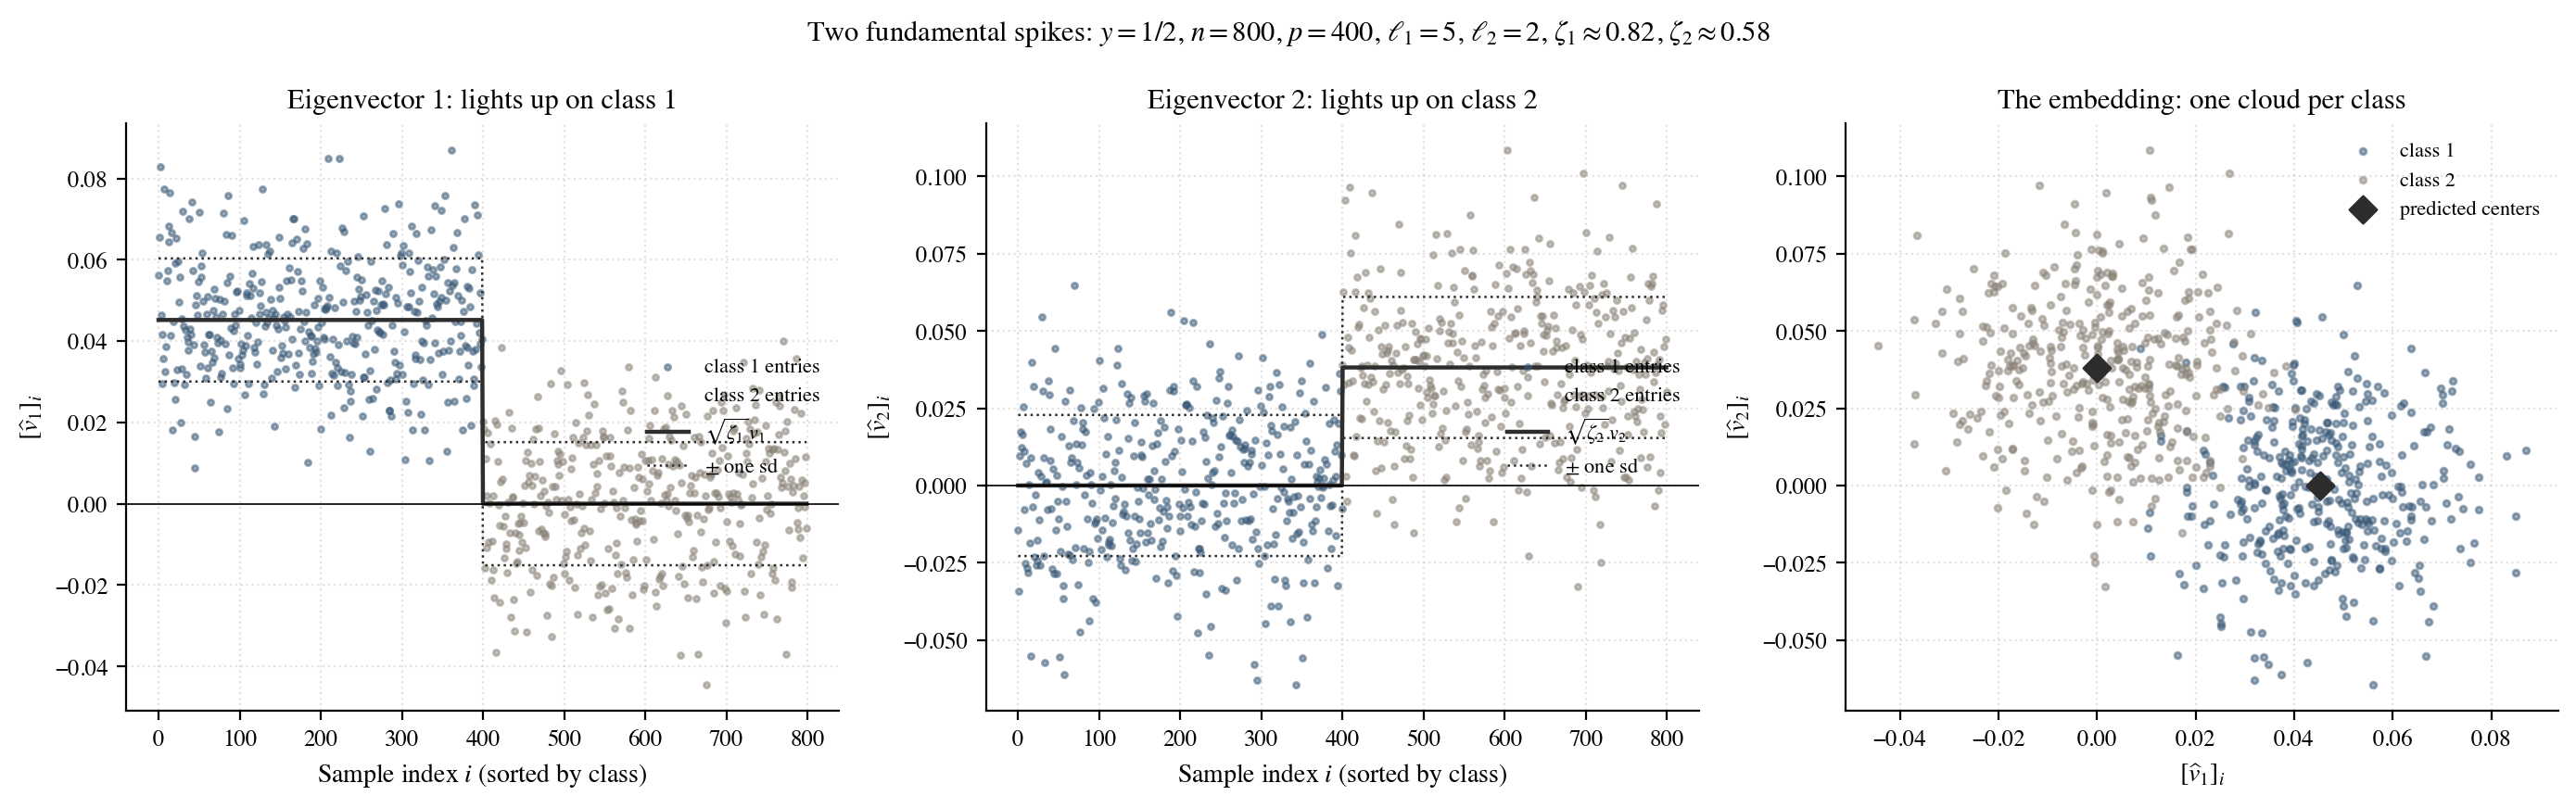
\includegraphics[width=\textwidth]{figures/clustering_two_spikes.png}
  \caption{Two fundamental spikes at \(y = 1/2\), \(n = 800\), \(p = 400\), \(\ell_1 = 5\), \(\ell_2 = 2\) (one realization). \emph{Left and middle:} entries of the top two eigenvectors; each tracks its own normalized indicator, shrunk by \(\sqrt{\zeta_k}\) (solid) within the predicted band (dotted), and stays at zero on the other group. \emph{Right:} the spectral embedding: each point is an observation plotted at \(([\widehat{\vect{v}}_1]_i, [\widehat{\vect{v}}_2]_i)\); the two groups form two Gaussian clouds at the predicted centers (diamonds). Generated by \texttt{notebooks/05\_clustering\_demos.py}.}
  \label{fig:clustering-two-spikes}
\end{figure}

\paragraph{The clustering phase transition.}
Finally, the threshold itself. Figure~\ref{fig:clustering-accuracy} sweeps the signal-to-noise ratio \(\ell\) through \(\sqrt{y}\) in the two-group problem and records the fraction of points classified correctly by the sign rule. Below the threshold the eigenvector is noise (Section~\ref{subsec:eigenvector}'s delocalization, now seen on the Gram matrix) and the accuracy sits at the coin-flip level \(1/2\); above it, the accuracy follows the predicted curve \(\Phi(\sqrt{\zeta/(1-\zeta)})\) toward \(1\). This is the phase transition of Section~\ref{subsec:bbp} in applied form: the same algebra that decided when an eigenvalue escapes the bulk decides when a dataset can be clustered at all.

\begin{figure}[H]
  \centering
  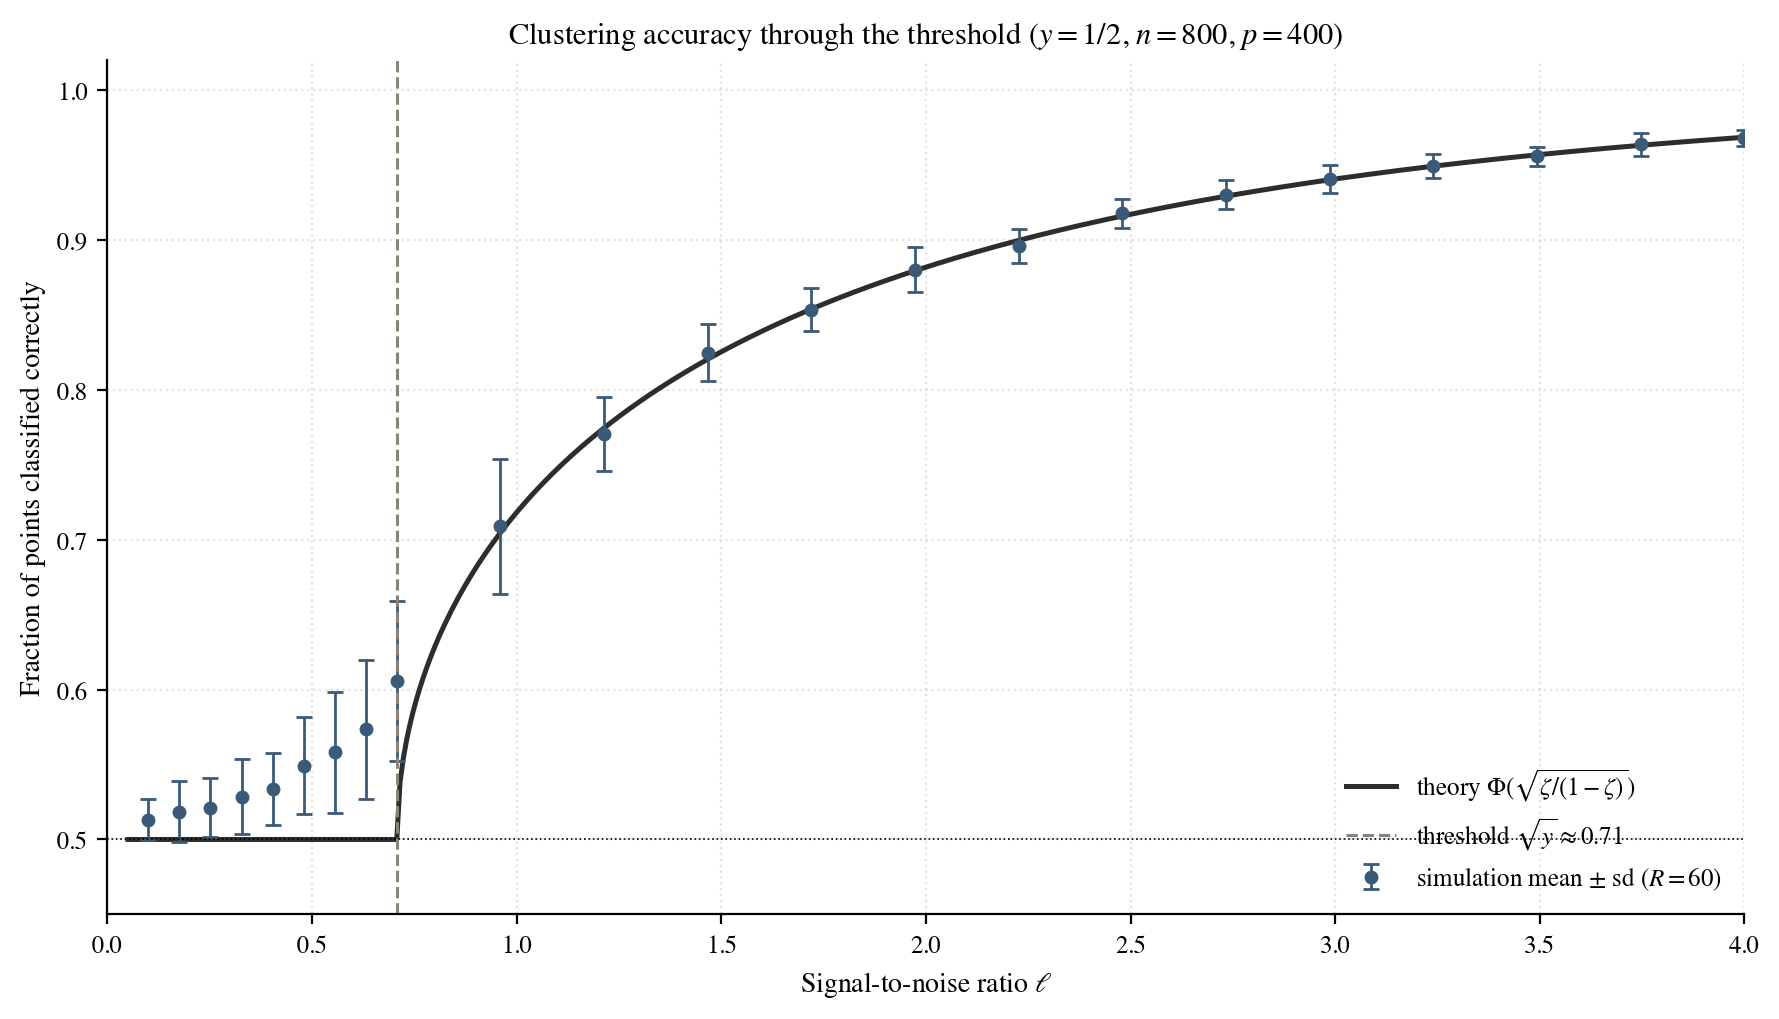
\includegraphics[width=0.85\textwidth]{figures/clustering_accuracy_transition.png}
  \caption{Fraction of points clustered correctly against the signal-to-noise ratio \(\ell\), at \(y = 1/2\), \(n = 800\), \(p = 400\), with \(R = 60\) replications per point (mean \(\pm\) one standard deviation). Below the threshold \(\sqrt{y} \approx 0.71\) (dashed) the accuracy is a coin flip; above it, it climbs along the predicted law \(\Phi(\sqrt{\zeta/(1-\zeta)})\) of~\eqref{eq:sign-accuracy}. Generated by \texttt{notebooks/05\_clustering\_demos.py}.}
  \label{fig:clustering-accuracy}
\end{figure}

\subsection{Spectral Clustering in Practice: Handwritten Digits}\label{subsec:mnist}

The clustering theory of Section~\ref{subsec:clustering} was proved, and simulated, under a Gaussian model.\gdmark{r4-mnist-exact} Real data obey no such model, and images in particular are conspicuously non-Gaussian, which makes them a genuine test.\gdmark{r4-nongaussian} The accuracy prediction should survive anyway, for a reason built into the proof of Theorem~\ref{thm:eigvec-clt}: it used only that the noise has no preferred directions, not that it is Gaussian. This final subsection tests it on the MNIST dataset of handwritten digits \citep[e.g.,][]{LeCun1998}: seventy thousand grayscale images of the digits \(0\) through \(9\), each \(28 \times 28\) pixels. An image is a vector \(\vect{x}_i \in \R^{784}\) of pixel intensities scaled to \([0, 1]\), so \(p = 784\), and the cluster means are the average shapes of the ten digits.

\paragraph{Two digits.}
We start with the cleanest pair, \(0\) versus \(1\), taking \(6{,}000\) images of each (\(n = 12{,}000\)). The procedure is the one verified in Figure~\ref{fig:clustering-one-spike},\gdmark{r4-procedure} following the published code of \citet{LebeauChatelainCouillet2024}: form the Gram matrix, take its top eigenvector \(\widehat{\vect{v}}\), and read the two groups from the signs of its entries. (The eigenvector is first centered and renormalized, since all images share a large average shape that the raw eigenvector would otherwise track instead of the digit contrast.) The true labels are used only to \emph{score} the result, never to form it:\gdmark{r4-evaluate} with \(\vect{v}\) the normalized label contrast (entries \(\pm 1/\sqrt{n}\)), the alignment is estimated as \(\widehat{\zeta} = \abs{\inner{\vect{v}}{\widehat{\vect{v}}}}^2\), and Theorem~\ref{thm:eigvec-clt} predicts everything else with no free parameters. Figure~\ref{fig:mnist-zero-one} shows the result: the eigenvector entries form the two predicted bands, the residuals match the predicted Gaussian \(\Normal{0, (1 - \widehat{\zeta})/n}\), and with \(\widehat{\zeta} \approx 0.703\) the predicted accuracy \(\Phi(\sqrt{\widehat{\zeta}/(1-\widehat{\zeta})}) \approx 0.938\) sits against an observed \(0.934\). A theorem proved for an idealized spiked model predicts the error rate on real handwriting to within half a percentage point. This is a small instance of a broad phenomenon: random-matrix predictions calibrated on Gaussian models track real-data performance closely, evidence that the outcome depends on the data only through its second-order statistics \citep{CouilletLiao2022}.\gdmark{r4-universality}

\begin{figure}[H]
  \centering
  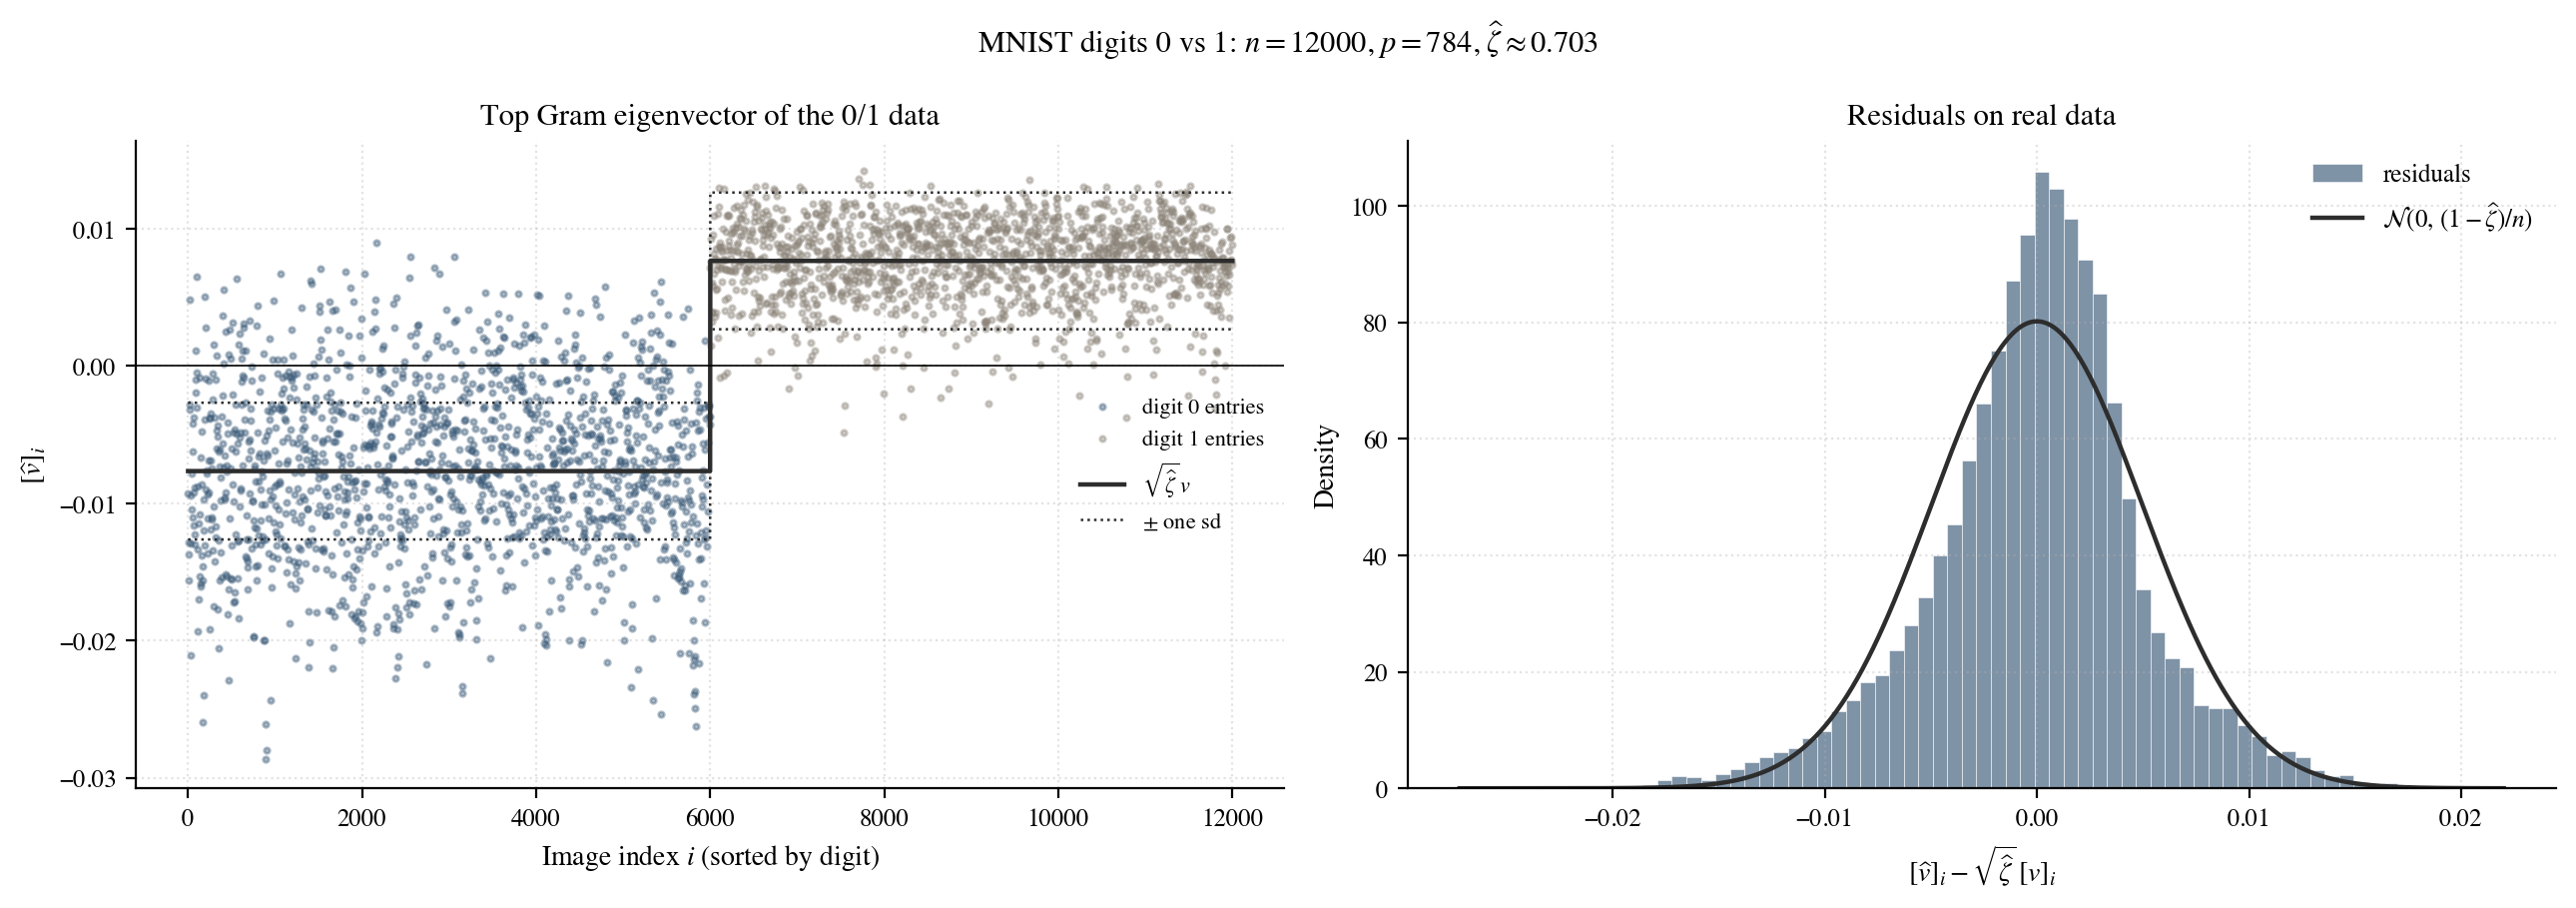
\includegraphics[width=\textwidth]{figures/mnist_zero_one.png}
  \caption{MNIST digits \(0\) versus \(1\) (\(n = 12{,}000\), \(p = 784\)). \emph{Left:} entries of the top Gram eigenvector, one per image, sorted by digit; the solid line is the prediction \(\sqrt{\widehat{\zeta}}\, \vect{v}\) with \(\widehat{\zeta} \approx 0.703\) estimated from the data, the dotted lines the one-standard-deviation band of Theorem~\ref{thm:eigvec-clt}. \emph{Right:} the residuals against the predicted \(\Normal{0, (1-\widehat{\zeta})/n}\); the curve is this prediction, not a fit.\gdmark{r4-fit} Generated by \texttt{notebooks/05\_clustering\_demos.py}.}
  \label{fig:mnist-zero-one}
\end{figure}

\paragraph{All forty-five pairs.}
Repeating this for every pair of digits gives Figure~\ref{fig:mnist-pairs}, which places the observed accuracy (the fraction correctly sorted, upper triangle) beside the predicted accuracy~\eqref{eq:sign-accuracy} (lower triangle) for all \(45\) two-digit problems.\gdmark{r4-pairs} The two agree closely across the board: the mean absolute gap is \(0.004\) and the worst is \(0.015\). The matrix is, in effect, a difficulty map of MNIST as seen by the identity kernel. Pairs involving the visually distinctive \(1\) are easiest, with \(0\)/\(1\) at \(0.93\); the pairs \(2\)/\(3\), \(2\)/\(6\), and \(4\)/\(7\) sit at \(0.50\) to \(0.51\), genuine coin flips, because their mean images are too alike for the signal-to-noise ratio \(\ell\) to clear the threshold \(\sqrt{y}\). The theory explains these numbers rather than merely fitting them:\gdmark{r4-negation} each cell is a Gaussian tail \(\Phi(\sqrt{\widehat{\zeta}/(1-\widehat{\zeta})})\), so a pair is hard precisely when its alignment \(\widehat{\zeta}\) is near zero.

\begin{figure}[H]
  \centering
  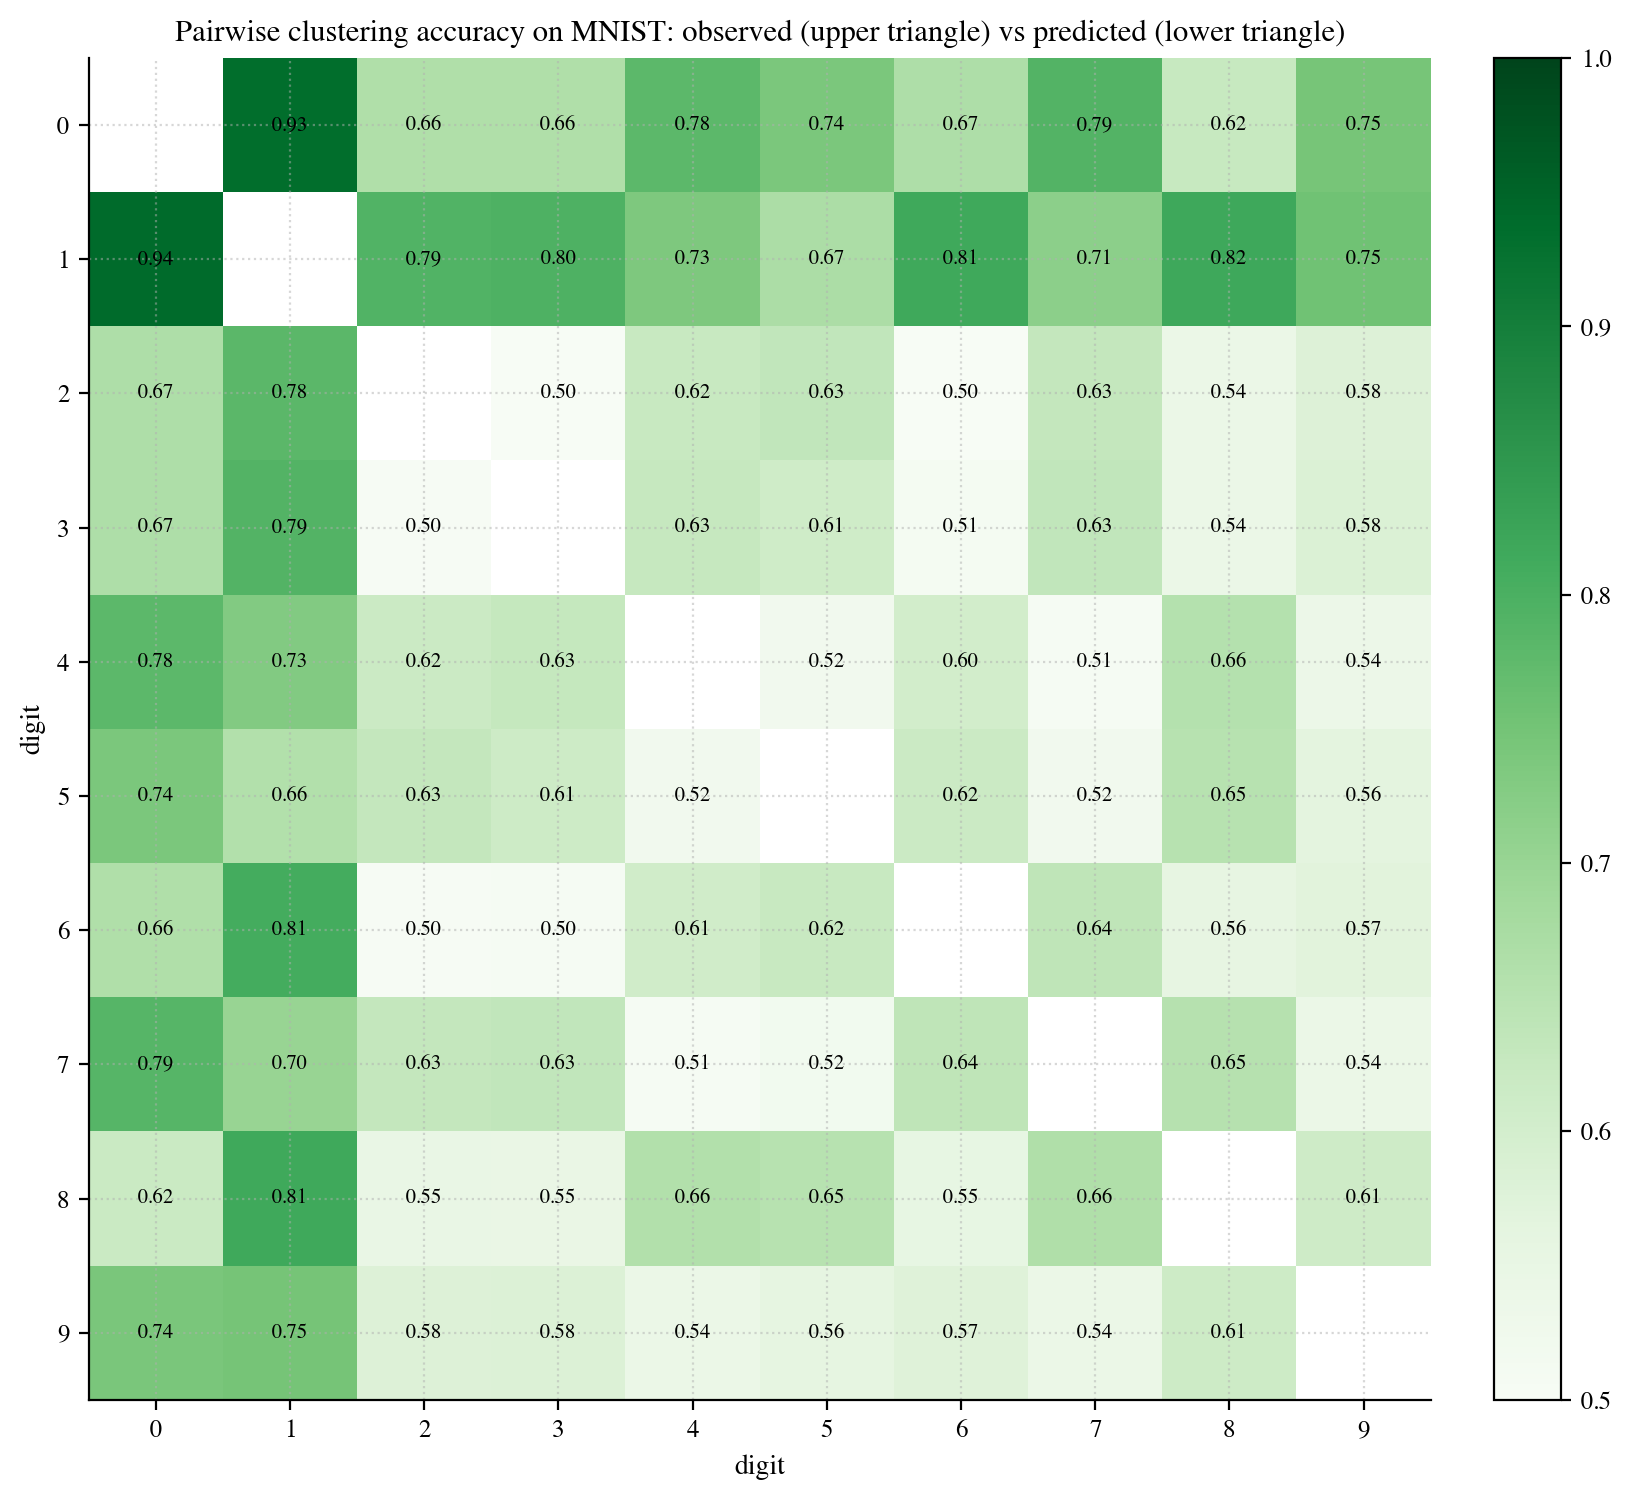
\includegraphics[width=0.8\textwidth]{figures/mnist_pairs_heatmap.png}
  \caption{Two-digit spectral clustering accuracy for all \(45\) MNIST pairs (\(5{,}400\) images per digit). Upper triangle: observed fraction of correctly clustered images. Lower triangle: the prediction \(\Phi(\sqrt{\widehat{\zeta}/(1-\widehat{\zeta})})\) of~\eqref{eq:sign-accuracy}. The mean absolute difference between the two triangles is \(0.004\).\gdmark{r4-pairs-caption} Generated by \texttt{notebooks/05\_clustering\_demos.py}.}
  \label{fig:mnist-pairs}
\end{figure}

\paragraph{All ten digits.}
Finally, the full problem: cluster all ten digits at once (\(5{,}400\) images per digit, \(n = 54{,}000\)). Each image is mapped to its entries in the top nine eigenvectors of the Gram matrix (computed after removing the mean image), giving a point in nine dimensions, and \(k\)-means groups those points into ten clusters by proximity.\gdmark{r4-embedded} Nine eigenvectors suffice for ten classes because the ten indicator vectors are not independent: they sum to the constant vector, and removing the mean image deletes exactly that direction, leaving the \(K - 1 = 9\) dimensions of genuine between-class contrast (the same reason each two-digit problem needed only one centered eigenvector).\gdmark{r4-ninedim} The cluster labels are matched to digits, for scoring only, by the assignment that maximizes agreement. Figure~\ref{fig:mnist-ten-class} reports the outcome: \(53\%\) of the \(54{,}000\) images land in the right cluster, against \(10\%\) for random guessing.

\begin{figure}[H]
  \centering
  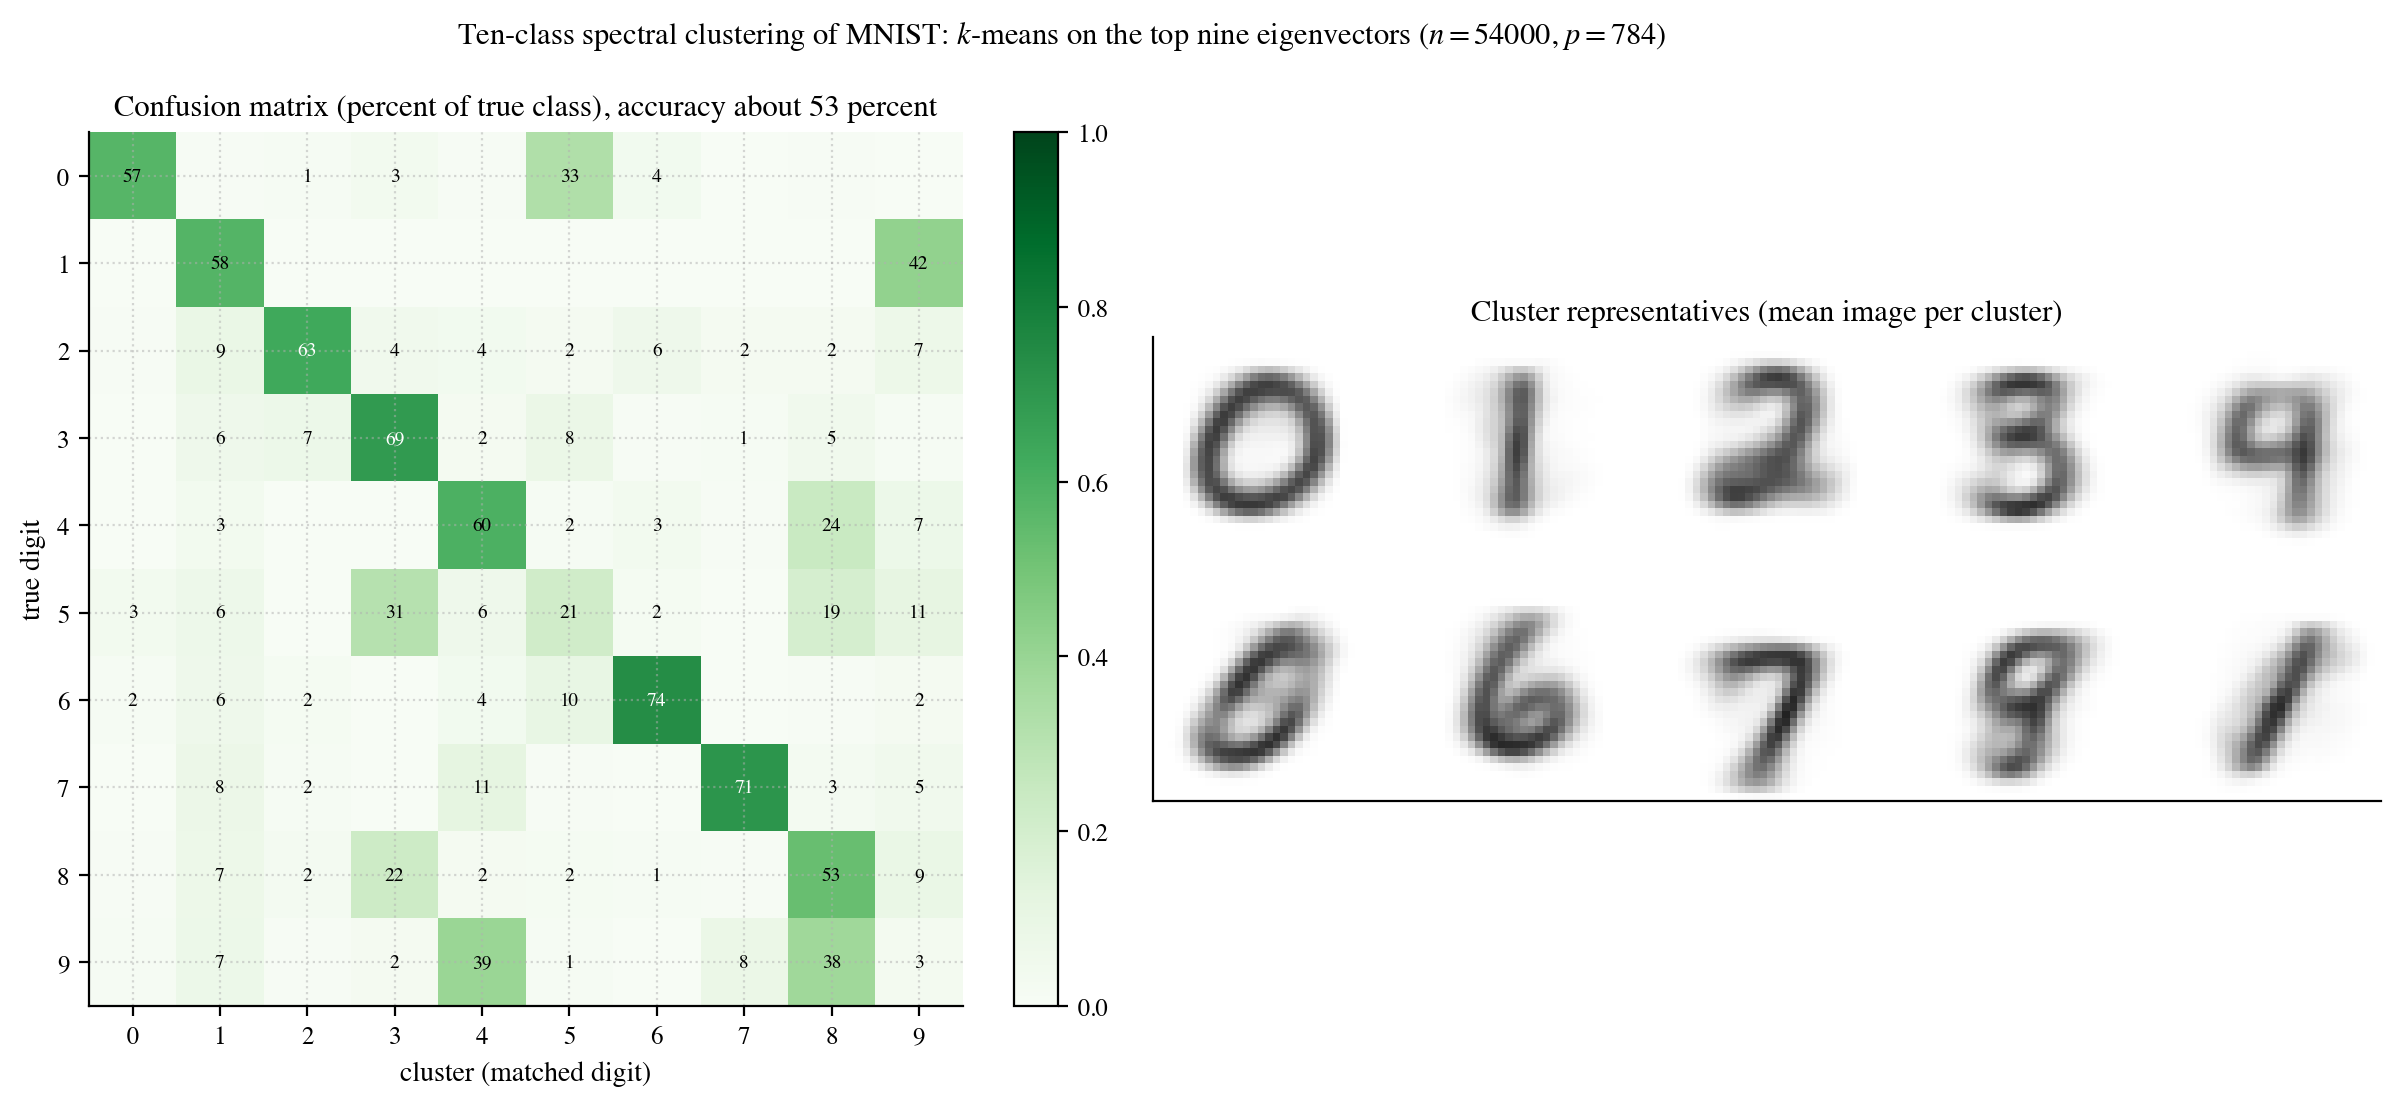
\includegraphics[width=\textwidth]{figures/mnist_ten_class.png}
  \caption{Ten-class spectral clustering of MNIST: \(k\)-means on the top nine Gram eigenvectors (\(n = 54{,}000\), \(p = 784\)). \emph{Left:} confusion matrix (rows: true digit; columns: matched cluster; entries: percent of the true class), overall accuracy \(\approx 53\%\). \emph{Right:} the mean image of each cluster: the algorithm has discovered recognizable digit shapes without ever seeing a label. Generated by \texttt{notebooks/05\_clustering\_demos.py}.}
  \label{fig:mnist-ten-class}
\end{figure}

The confusion matrix and the difficulty map of Figure~\ref{fig:mnist-pairs} tell one consistent story. The digits that clustering recovers well (\(6\) at \(74\%\), \(7\) at \(71\%\), \(3\) at \(69\%\)) are those whose rows in the pairwise map are mostly easy, and the failures are exactly the predicted ones: digit \(9\), whose pairwise accuracy against \(4\) is \(0.54\) and against \(7\) is \(0.54\) (alignments \(\widehat{\zeta} \approx 0.01\)), is essentially never given its own cluster, because in the embedding its cloud sits on top of those of \(4\) and \(7\). These failures are not algorithmic accidents; they are information limits \emph{of this similarity matrix}. The identity kernel sees only the average shapes of the digits, and where average shapes nearly coincide, Theorem~\ref{thm:gram-spikes} says the relevant spike is below threshold and no method based on the top eigenvectors of \(\mat{G}\) can do better. Nonlinear kernels change the similarity, and hence the signal-to-noise ratios, which is how richer methods push past this limit \citep{CouilletBenaych2016}.\gdmark{r4-practical}

\paragraph{The PCA connection.}
Readers who know some machine learning will recognize the embedding step: the top eigenvectors of the Gram matrix \((1/p)\mat{X}\transpose\mat{X}\) are, up to scale, the top \emph{principal component scores} of the data, so the procedure of this subsection is ``run \(k\)-means on the first few principal components,'' one of the oldest recipes in applied data analysis. In that light, Sections~\ref{sec:scm} through~\ref{sec:clustering} together form the theory of when that recipe works: Section~\ref{sec:scm} described what the components look like when there is nothing to find, Sections~\ref{subsec:johnstone}--\ref{subsec:two-spikes} located the threshold a signal must clear before a component carries information and quantified how much of it is recovered, and Theorems~\ref{thm:gram-spikes} and~\ref{thm:eigvec-clt} priced the residual noise down to the accuracy of the final clustering.

\clearpage
